\documentclass[letterpaper,10pt]{article}

\usepackage{titling}
\usepackage{listings}
\usepackage{url}
\usepackage{setspace}
\usepackage{subfig}
\usepackage{sectsty}
\usepackage{pdfpages}
\usepackage{colortbl}
\usepackage{multirow}
\usepackage{relsize}
\usepackage{amsmath}
\usepackage{fancyvrb}
\usepackage{amsmath,amssymb,amsthm,graphicx,xspace}
\usepackage[titlenotnumbered,noend,noline]{algorithm2e}
\usepackage[compact]{titlesec}
\usepackage[default]{droidserif}
\usepackage[T1]{fontenc}
\usepackage{tikz}
\usetikzlibrary{arrows,automata,shapes,trees,matrix,chains,scopes,positioning,calc}
\tikzstyle{block} = [rectangle, draw, fill=blue!20, 
    text width=2.5em, text centered, rounded corners, minimum height=2em]
\tikzstyle{bw} = [rectangle, draw, fill=blue!20, 
    text width=4em, text centered, rounded corners, minimum height=2em]

\definecolor{namerow}{cmyk}{.40,.40,.40,.40}
\definecolor{namecol}{cmyk}{.40,.40,.40,.40}

\let\LaTeXtitle\title
\renewcommand{\title}[1]{\LaTeXtitle{\textsf{#1}}}


\newcommand{\handout}[5]{
  \noindent
  \begin{center}
  \framebox{
    \vbox{
      \hbox to 5.78in { {\bf ECE155: Engineering Design with Embedded Systems } \hfill #2 }
      \vspace{4mm}
      \hbox to 5.78in { {\Large \hfill #4  \hfill} }
      \vspace{2mm}
      \hbox to 5.78in { {\em #3 \hfill} }
    }
  }
  \end{center}
  \vspace*{4mm}
}

\newcommand{\lecture}[3]{\handout{#1}{#2}{#3}{Lecture #1}}
\newcommand{\tuple}[1]{\ensuremath{\left\langle #1 \right\rangle}\xspace}

\addtolength{\oddsidemargin}{-1.000in}
\addtolength{\evensidemargin}{-0.500in}
\addtolength{\textwidth}{2.0in}
\addtolength{\topmargin}{-1.000in}
\addtolength{\textheight}{1.75in}
\addtolength{\parskip}{\baselineskip}
\setlength{\parindent}{0in}
\renewcommand{\baselinestretch}{1.5}
\newcommand{\term}{Spring 2014}

\singlespace


\begin{document}

\lecture{ 16 --- Code Coverage and Testing on Android}{\term}{Jeff Zarnett and Patrick Lam}

\section*{Code Coverage}
To get an idea of how well our test cases are testing the program, we can consider a concept called \textit{code coverage}. In simple terms, we want to know what lines of the program are executed during our tests. Covering lines in a sequential program is one thing, but all non-trivial programs have some logic to them that involves conditionals (if statements, for example). 

A conditional is any statement which will be evaluated to true or false, and then the evaluated value is used to decide what the next step is. As an example: \texttt{if (x == 0) \{ foo(); \} else \{ bar(); \} }. When execution reaches the if-statement, x is compared to 0 and this returns a value of true or false. If it is true, then the next statement to be run will be the function call to \texttt{foo()}; otherwise the next statement will be the function call to \texttt{bar()}.

There are some different definitions for coverage~\cite{pantest}:
\begin{itemize}
	\item \textbf{Statement Coverage} -- executing each line of code at least once;
	\item \textbf{Branch Coverage} -- traverse each branch (conditional) statement; and
	\item \textbf{Multiple Condition Coverage} -- cover all possible combinations of the conditional statements.
\end{itemize}

We say a line is ``covered'' if that line is executed during the course of the test cases. A branch is covered if that branch is executed during the course of the test cases. In multiple condition coverage, we might say a class or module is covered if all combinations of the conditionals within it are tested.

Whichever method we choose, we want to have an idea about how much of the software under examination is being tested by the test cases. We will focus mostly on line coverage in this course. Getting 100\% statement coverage is generally unrealistic, but even if it is achieved, it does not guarantee that the software is bug-free. A statement that divides two numbers may perform well in the test cases, but badly if the user inputs a zero (resulting in a division by zero error). 

Code coverage testing might reveal some ``dead code'' -- code that can never be executed. In simple cases, the compiler will detect for you that a block of code is unreachable, but more complex situations might only be revealed by looking at the execution of the program under test. Dead code plays no real role in the system, except that programmers might be making unnecessary effort to maintain it when it could be removed altogether. 

As test cases are added, we will start to encounter diminishing returns. The first test is all ``new'' lines being tested. Up to a point it may be possible to add more completely independent tests. Once a baseline of tests is established, additional tests will add fewer lines to the body of covered lines. 

\subsection*{Case Study: EclEmma}
As our case study, we will examine a plug-in for Eclipse called EclEmma. This does not come as part of Eclipse by default, but can be installed in the environment easily. Images in this section come from \texttt{http://www.eclemma.org}, the official EclEmma site.

When launched, EclEmma runs the selected unit tests and then analyzes the results. The results are presented in two ways; the first of which is source highlighting. EclEmma will colour-code each line in either:
\begin{itemize}
	\item \textbf{Red} -- the line was not executed;
	\item \textbf{Yellow} -- a conditional where only one branch was taken (e.g., an if was always evaluated as false); or
	\item \textbf{Green} -- the line was executed, or in the case of a conditional, both branches were taken.
\end{itemize}

\begin{center}
	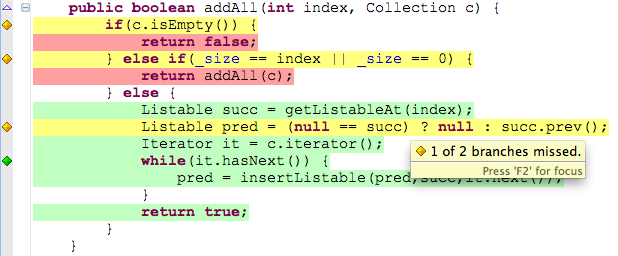
\includegraphics[width=0.75\textwidth]{images/annotations.png}
\end{center}

In addition to colour-coding the lines, EclEmma will provide a report that shows how much is tested (by percentage) in each file and package.

\begin{center}
	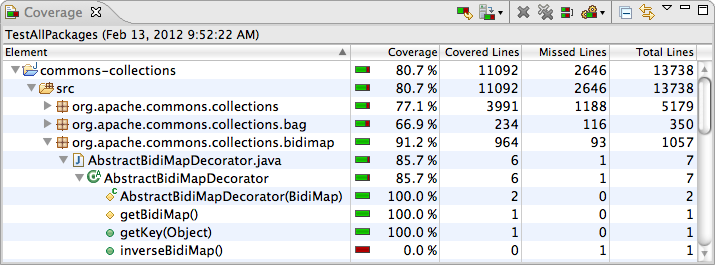
\includegraphics[width=\textwidth]{images/coverageview.png}
\end{center}

Using the coverage data, you can decide if your tests are effective in testing the logic of the code. Too many red lines in the project means more tests (or better tests) are needed.

\subsection*{Example: Testing \texttt{computeValue}}

Recall that in Code Coverage Analysis, each line of a method containing logic or a statement (that is, not just a \texttt{\}} brace) is colour-coded:
\vspace{-1em}
\begin{itemize}
\item Red: if the line was not executed;
\item Yellow: if the line is a conditional where only one branch was taken;
or
\item Green: if the line was executed, or in the case of a conditional, both branches were taken.
\end{itemize}
\vspace{-1em}
To the left of each line of code of the function \texttt{computeValue}, indicate whether it is coded as green (G), yellow (Y), or red (R) at the end of all tests (cumulative results) if the JUnit tests invoke the method as \texttt{computeValue(7, -1)} and \texttt{computeValue(0, 1000)}.

\begin{verbatim}
public double computeValue(int input1, int input2) {
  if (input1 < 0) {
    throw new IllegalArgumentException(``Input 1 may not be negative'');
  }
  
  if (input2 == -1) {
    return 0;
  } else if (input2 <= 1) {
    return 1;
  }
 
  int result = (input1 * input2); 
  result += (input1 / input2);
  
  return result;

}
\end{verbatim}

\paragraph{Solution:}

\begin{verbatim}
public double computeValue(int input1, int input2) {
Y  if (input1 < 0) {
R    throw new IllegalArgumentException(``Input 1 may not be negative'');
   }
  
G  if (input2 == -1) {
G    return 0;
Y  } else if (input2 <= 1) {
R    return 1;
  }
 
G  int result = (input1 * input2); 
G  result += (input1 / input2);
  
G  return result;
}
\end{verbatim}




\section*{Testing for Android}


The course is about embedded systems, so we'll take some time to examine testing of embedded systems in the context you are now most familiar with: Android.


It's easy if you
test classes that don't use the operating system.  This is good program design
anyway: split the Android-dependent parts from the general parts. Do
that, when possible. 

For the purpose of this course, you could put the step recognition
code in a separate class and call it from the Activity. That would be
a first step towards a Model-View-Controller design.

However, if you want to test the Android-specific parts of your app,
you'll need something to call those parts, because Android apps are
event-driven. We'll talk about what Android provides for test automation.
Note that this is not really a unit test. Despite its name, JUnit isn't just
for writing unit tests. You can also use it for integration tests.

\paragraph{What To Test.}
You can test these aspects of your app manually; however, it's better to have a test
script for them~\cite{android:testwhat}.

Orientation change:
\begin{itemize}
\item is screen redrawn correctly?
\item did you lose any state?
\end{itemize}

Configuration change (e.g. adding a keyboard):
\begin{itemize}
\item again as for orientation change;
\item do you handle the new device properly?
\end{itemize}

Battery life:
\begin{itemize}
\item don't hog the battery (out of scope for us).
\end{itemize}

External resources:
\begin{itemize}
\item how does your app behave when it doesn't have
necessary resources, e.g. GPS?
\end{itemize}

We'll continue by talking about how to test Android apps.


\section*{Android Activity Unit Tests.} It is allegedly possible to test an
{\tt Activity} in isolation using the {\tt ActivityUnitTestCase}. That
would be more in the spirit of unit tests. However, I couldn't
actually find useful tutorials about how to do that, so I'll just say
that it's beyond the scope of this course.

\subsection*{Android Integration Test Cases.}
The basic idea here is that a test case is a set of program inputs and
expected program outputs. While it is possible to do this manually,
that would restrict our ability to inspect program state, unless the
program had debug statements (which consume resources and are tedious
to manually verify).

We'd instead like to automate Android testing. Use {\tt ActivityInstrumentationTestCase2}\footnote{This is terrible naming!}.

Creating an Android integration test case takes quite a few steps.
Basically, you create a new project and make it call the app that
you're trying to test. The test case and the app are closely tied together.

A general reference to Android testing is here:

\begin{center}
{\url{http://developer.android.com/tools/testing/activity_testing.html}}
\end{center}

It is too generic, though. A more useful (but overly-long) tutorial is here:

\begin{center}
{\url{http://developer.android.com/tools/testing/activity_test.html}}
\end{center}

However, that tutorial is too long for us to go over in class. But if you are really interested, the appendix to this lecture has some highlights.


\subsection*{Case Study: QA for Android Games}
Let's make it real by discussing a case study of Android game QA~\cite{techcrunch}.

Android phones have a lot of fragmentation: there are literally hundreds of different devices out there, made by different manufacturers, with different specifications. A Hong Kong developer, Animoca, tests on about 400 different phones and tablets. This is a lot, but this is easy in comparison to the era of what were called ``feature phones'' -- when just about every phone was unique. Android provides at least \emph{some} standardization.

\paragraph{Test On Real Devices.} Emulators are good, but they're not always perfect. 
If you really care about quality, or if you want to handle sensor input, you will need
to test on real devices. In the labs, we work with sensor data, so emulators are not very useful. Games that rely on touch input and so on are also difficult to test with an emulator. 

\paragraph{Choosing Devices to Test On.} You need to figure out how many devices to test on; many developers test on a small number (e.g. 5 or 12) of devices, which will cover many combinations. Some areas to consider: tablet vs phone, high-res screen vs low-res screen, what kind of GPU, etc. Individual devices which are very popular (e.g., the Samsung Galaxy S3) are good choices to test with.


\paragraph{Know What \emph{Not} to Test.} In addition to figuring out what devices you will test on, you also have to consider what you will not support. You may choose to say no to small, slow, or outdated phones and operating systems. It will not be possible to support every single Android device in the world, so focus your testing effort where it gets the most ``bang for the buck''. It's often better to choose not to support a low-end device (or old OS) than it is to test your app on a phone that's owned by 4 people in the world (or worse... release your software untested).

\paragraph{Test Continuously.} Pocket Gems makes Android games. They create
and perform tests, and then offshore the rest of the testing. The offshore 
testing team files bugs in the bug tracker, which go back to the US. Tests are also created concurrently with the development of the software, so that when features are ready they can be tested immediately.

\paragraph{Test Coverage.} In Android devices, and embedded systems in general, it's not enough to check the features of the software. Memory is limited, as is processing power and battery life. So memory use, performance, and battery life all need to be tested.

Testing is tightly integrated with development. You can't test at the end
and hope to succeed. Testing everything all at the end is known as ``big bang testing'', and is not likely to work.

They also run a final test phase before shipping code. That phase is expensive
and thorough, checking memory, performance, and device compatibility.




\section*{Appendix: Android Activity Testing}

Note that this appendix section is not considered testable material for exams; it is here only for your reference and possible interest.

\paragraph{Creating a Test Project.} 
After you have your main app project, you need a test project as well.
Create a new project with File \textgreater\- New \textgreater\- Other
and choose ``New Android Test Project''. If I called my original package
{\tt ca.patricklam.ece155.A4}, I should call the test package {\tt
ca.patricklam.ece155.A4.text}.

You should now have both the Android activity and the test project. The
test project should currently be empty.

\paragraph{Creating a Test Project Class.} 
Next, you need to actually create a test class and populate it with
test methods.  This is a new class that you create in the test
project, e.g. {\tt DatePickerActivityTest}.  Add it with File
\textgreater\- New \textgreater\- Class.  

\begin{itemize}
\item The superclass needs to be \verb+ActivityInstrumentationTestCase2<DatePickerActivity>+.
\end{itemize}

In that class, you'll need a
constructor, a setup method, and test methods.

\paragraph{Constructor.} For technical reasons, your test class needs a constructor with the
package name and class of the activity under test:

{\small
\begin{verbatim}
  public DatePickerActivityTest() {
    super("ca.patricklam.ece155.A4", DatePickerActivity.class);
  }
\end{verbatim}
}

\paragraph{Setup method.} Unlike the constructor, the setup method may run many times.
It needs to set up the infrastructure for the test cases. Here's an example:

{\small
\begin{verbatim}
  // fields for objects under test
  private DatePickerActivity activityUnderTest;
  private TextView monthViewUnderTest;
  private Button okButton;
  private Instrumentation instrumentation;

  // name must be setUp() for JUnit 3, as used by Android.
  @Override
  protected void setUp() throws Exception {
    super.setUp();

    // if this is missing, any key events you send will be ignored
    setActivityInitialTouchMode(false);
    activityUnderTest = getActivity();
    monthViewUnderTest = (TextView) activityUnderTest.findViewById
                                      (ca.patricklam.ece155.A4.R.id.month);
    okButton = (Button) activityUnderTest.findViewById
                                      (ca.patricklam.ece155.A4.R.id.button);

    // lets you control the test object
    instrumentation = getInstrumentation();
  }
\end{verbatim}
}

\paragraph{Test Cases.} Now you can use JUnit infrastructure to write test cases.
This is a bit tricky due to the UI thread issue we encountered last time.
Anything you do to the activity UI has to be in a {\tt runOnUiThread()} block,
just like with the {\tt Timer}. You can also send keys and wait for the activity
to finish chugging along. Finally, you'll want assertions.

{\small
\begin{verbatim}
  public void testBadMonth() {
    // clear state of month textview
    activityUnderTest.runOnUiThread(
      new Runnable() {
        public void run() {
          monthViewUnderTest.setText("");
          monthViewUnderTest.requestFocus();
        }
      });

    // try to insert "13" in the month
    this.sendKeys(KeyEvent.KEYCODE_1);
    this.sendKeys(KeyEvent.KEYCODE_3);
    this.sendKeys(KeyEvent.KEYCODE_ENTER);

    // let it process the key events
    instrumentation.waitForIdleSync();

    // payload: check to see that the field rejects the entry
    assertFalse("text field not 13", 
                monthViewUnderTest.getText().toString().equals("13"));
  }
\end{verbatim}
}

At this point, you can test your test and see if it works. If you're using
Test-Driven Development, you'd build the test first, see that it fails,
and then fix the code. To run it, just select the test project and run that.

\paragraph{Other Things to Test.}
The tutorial also suggests verifying the state of the Activity before
you do anything. That's a good idea.


\bibliographystyle{alpha}
\bibliography{155}


\end{document}
